
		\documentclass[a4paper]{article}
		
		%package include
		\usepackage[margin=3cm]{geometry}
		\usepackage[italian]{babel}
		\usepackage[utf8]{inputenc}
		\usepackage[T1]{fontenc}
		\usepackage{graphicx}
		\usepackage{fancyhdr}
		\usepackage{lastpage}
		\usepackage{longtable}
		\usepackage{tabu}
		\usepackage{hyperref}
		\usepackage[hypcap]{caption}
		\usepackage{color}
		\usepackage{xcolor}
		\usepackage{eurosym}
		\usepackage{abstract}
		\usepackage{float}
		\usepackage{listings, lstautogobble}
		\usepackage{amsmath}
		\usepackage{subfigure}
		\usepackage{pifont}
		\usepackage{multirow}

		\colorlet{punct}{red!60!black}
		\definecolor{background}{HTML}{EEEEEE}
		\definecolor{delim}{RGB}{20,105,176}
		\colorlet{numb}{magenta!60!black}


		% per allineare il codice a sinistra invece che al centro
		\lstset{
			autogobble=true,
			escapeinside={(*}{*)}
		}

		\lstdefinelanguage{json}{
		    basicstyle=\normalfont\ttfamily,
		    numbers=left,
		    numberstyle=\scriptsize,
		    stepnumber=1,
		    numbersep=8pt,
		    showstringspaces=false,
		    breaklines=true,
		    frame=lines,
		    backgroundcolor=\color{background},
		    literate=
		     *{0}{{{\color{numb}0}}}{1}
		      {1}{{{\color{numb}1}}}{1}
		      {2}{{{\color{numb}2}}}{1}
		      {3}{{{\color{numb}3}}}{1}
		      {4}{{{\color{numb}4}}}{1}
		      {5}{{{\color{numb}5}}}{1}
		      {6}{{{\color{numb}6}}}{1}
		      {7}{{{\color{numb}7}}}{1}
		      {8}{{{\color{numb}8}}}{1}
		      {9}{{{\color{numb}9}}}{1}
		      {:}{{{\color{punct}{:}}}}{1}
		      {,}{{{\color{punct}{,}}}}{1}
		      {\{}{{{\color{delim}{\{}}}}{1}
		      {\}}{{{\color{delim}{\}}}}}{1}
		      {[}{{{\color{delim}{[}}}}{1}
		      {]}{{{\color{delim}{]}}}}{1},
		}
		

		%macro definitions
		\newcommand{\groupname}{Kaizen Team}
\newcommand{\projectname}{Norris}

\newcommand{\proponente}{Maccagnan Alessandro}
\newcommand{\committente}{Vardanega Tullio}

\newcommand{\insglo}[1]{#1{\ped G}}
\newcommand{\ignoreglo}[1]{#1}
\newcommand{\insdate}[3]{#3-#2-#1}
\newcommand{\instime}[2]{#1-#2}
\newcommand{\insuri}[1]{\textcolor{blue}{\texttt{\url{#1}}}}
\newcommand{\inspath}[1]{\texttt{#1}}
\newcommand{\insrole}[1]{\textit{#1}}
\newcommand{\insdoc}[1]{\textit{“#1”}}
\newcommand{\insfile}[1]{“\texttt{#1}”}
\newcommand{\insrev}[1]{\textbf{#1}}
\newcommand{\insphase}[1]{\textbf{#1}}
\newcommand{\inslabel}[1]{\textit{“#1”}}

		\newcommand{\doctitle}{Definizione di Prodotto}
		\newcommand{\lastversion}{4.00}
		

		%abstract font
		\renewcommand{\abstractnamefont}{\huge\bfseries}
		\renewcommand{\abstracttextfont}{\large}

		%hyperred
		\hypersetup{
			linktoc=all,
			colorlinks=true,
			allcolors=black,
			urlcolor=blue,
			bookmarksdepth=100
		}

		%section counters
		\makeatletter
		\newcommand\level[1]{%
			\ifcase#1\relax\expandafter\chapter\or
				\expandafter\section\or
				\expandafter\subsection\or
				\expandafter\subsubsection\else
				\def\next{\@level{#1}}\expandafter\next
			\fi}
		\newcommand{\@level}[1]{%
			\@startsection{level#1}%
				{#1}%
				{\z@}%
				{-3.25ex\@plus -1ex \@minus -.2ex}%
				{1.5ex \@plus .2ex}%
				{\normalfont\normalsize\bfseries}}

		\newdimen\@numsdim
		\newdimen\@dotsdim
		{\normalfont\normalsize
			\sbox\z@{0}\global\@numsdim=\wd\z@
			\sbox\z@{.}\global\@dotsdim=\wd\z@
		}

		\newdimen\@numindent
		\newdimen\@textindent
		\setlength{\@numindent}{15pt}
		\setlength{\@textindent}{15pt}


		\newcounter{level4}[subsubsection]
		\@namedef{thelevel4}{\thesubsubsection.\arabic{level4}}
		\@namedef{level4mark}#1{}
		%\def\l@section{\@dottedtocline{1}{\dimexpr\@numindent*0\relax}{\dimexpr\@dotsdim*0+\@numsdim*1+\@textindent\relax}}
		\def\l@subsection{\@dottedtocline{2}{\dimexpr\@numindent*1\relax}{\dimexpr\@dotsdim*1+\@numsdim*2+\@textindent\relax}}
		\def\l@subsubsection{\@dottedtocline{3}{\dimexpr\@numindent*2\relax}{\dimexpr\@dotsdim*2+\@numsdim*3+\@textindent\relax}}
		\@namedef{l@level4}{\@dottedtocline{4}{\dimexpr\@numindent*3\relax}{\dimexpr\@dotsdim*3+\@numsdim*4+\@textindent\relax}}

		\count@=4
		\def\@ncp#1{\number\numexpr\count@+#1\relax}
		\loop\ifnum\count@<100
			\begingroup\edef\x{\endgroup
				\noexpand\newcounter{level\@ncp{1}}[level\number\count@]
				\noexpand\@namedef{thelevel\@ncp{1}}{%
					\noexpand\@nameuse{thelevel\@ncp{0}}.\noexpand\arabic{level\@ncp{1}}}
				\noexpand\@namedef{level\@ncp{1}mark}####1{}%
				\noexpand\@namedef{l@level\@ncp{1}}%
					{\noexpand\@dottedtocline%
						{\@ncp{1}}%
						{\dimexpr\@numindent*\@ncp{0}\relax}%
						{\the\dimexpr\@dotsdim*\@ncp{0}+\@numsdim*\@ncp{1}+\@textindent\relax}}}%
			\x
			\expandafter\edef\csname toclevel@level\the\count@\endcsname{\the\count@}%
			\advance\count@\@ne
		\repeat
		\makeatother
		
		\setcounter{tocdepth}{100}
		\setcounter{secnumdepth}{100}

		

		%fancyhdr config
		\fancyhf{}
		\fancyhead[L]{
\includegraphics[scale=0.05]{Pics/Logo} 
\includegraphics[height=7mm]{Pics/KaizenTeam}}
		\fancyhead[R]{\Large \bfseries \doctitle \vspace{0.1mm}}

		\fancypagestyle{roman}{
			\hypersetup{linkcolor=black}
			\pagenumbering{Roman}
			\fancyfoot[C]{\thepage{}}
		}

		\fancypagestyle{plain}{
			\hypersetup{linkcolor=blue}
			\pagenumbering{arabic}
			\fancyfoot[C]{\thepage{} di \pageref*{LastPage}}
		}

		
		%space between paragraph
		\raggedbottom
		


		\begin{document}

			\pagestyle{roman}
			\begin{titlepage}
  \begin{center}
	
	
\includegraphics{Pics/KaizenTeam} \\ [1cm]
	
	
\includegraphics[scale=0.6]{Pics/Logo} \\ [1cm]

	
\includegraphics[scale=0.3]{Pics/Norris} \\ [0.5cm]
	
\includegraphics[scale=1]{Pics/CoffeeStrap} \\ [2cm]

	
	\hrule
	\vspace{3mm}
	\Huge{\textbf{\doctitle{} v\lastversion{}}}
	\vspace{3mm}
	\hrule


	\vspace{2cm}

	\begin{minipage}{0.49\textwidth}
		\raggedright \large info@kaizenteam.it
	\end{minipage}
	\begin{minipage}{0.49\textwidth}
		\raggedleft \large \insuri{http://www.kaizenteam.it/}
	\end{minipage}

  \end{center}
\end{titlepage}

			\newpage
			

				\begin{center}
					\tabulinesep=6pt
					\begin{tabu} {X[r]|X[l]}
						\textbf{Versione} & 4.00 \\
						\textbf{Data redazione} & 2015-06-16 \\
						\textbf{Redazione} & \parbox[t]{0.4\textwidth}{Pavanello Fabio Matteo} \\
						\textbf{Verifica} & \parbox[t]{0.4\textwidth}{Dal Bianco Davide \\ Bucco Riccardo \\ Moretto Alessandro} \\
						\textbf{Approvazione} & \parbox[t]{0.4\textwidth}{Carlon Chiara} \\
						\textbf{Uso} & Esterno \\
						\textbf{Distribuzione} & \parbox[t]{0.4\textwidth}{\groupname{} \\ Prof. Vardanega Tullio \\ Prof. Cardin Riccardo \\ CoffeeStrap} \\
					\end{tabu}
				\end{center}

	
			\newpage
			
			\section*{Diario delle modifiche}
				\addtocounter{table}{-1}
				\tabulinesep=3pt
				\begin{longtabu} to \textwidth {|X[c,m]|X[c,m]|X[c,m]|X[c,m]|X[c,m]|}
					\hline
					\rowfont{\bf}
					Versione &
					Data &
					Autore &
					Ruolo &
					Descrizione \\
					\hline
					\endhead
					4.00 &
						2015-06-16 &
						Carlon Chiara &
						Project Manager &
						Approvazione del documento \\
						\hline
					3.06 &
						2015-06-14 &
						Dal Bianco Davide &
						Verificatore &
						Verifica descrizioni \\
						\hline
					3.05 &
						2015-06-13 &
						Pavanello Fabio Matteo &
						Progettista &
						Aggiunta descrizione diagrammi di sequenza \\
						\hline
					3.04 &
						2015-06-12 &
						Bucco Riccardo &
						Verificatore &
						Verifica incremento \\
						\hline
					3.03 &
						2015-06-12 &
						Pavanello Fabio Matteo &
						Progettista &
						Unione sezione classi aggiuntive con classi \\
						\hline
					3.02 &
						2015-06-11 &
						Moretto Alessandro &
						Verificatore &
						Verifica contenuto diagrammi  \\
						\hline
					3.01 &
						2015-06-10 &
						Pavanello Fabio Matteo &
						Progettista &
						Modifica descrizioni dei diagrammi \\
						\hline
					3.00 &
						2015-05-12 &
						Pavanello Fabio Matteo &
						Project Manager &
						Approvazione del documento \\
						\hline
					2.02 &
						2015-05-12 &
						Moretto Alessandro &
						Verificatore &
						Verifica contenuto diagrammi  \\
						\hline
					2.01 &
						2015-05-11 &
						Bigarella Chiara &
						Progettista &
						Creazione diagrammi con Astah per l'importazione automatica nella sezione “Specifica dei componenti” implementando i requisiti opzionali \\
						\hline
					2.00 &
						2015-05-26 &
						Bigarella Chiara &
						Project Manager &
						Approvazione del documento \\
						\hline
					1.02 &
						2015-04-25 &
						Bucco Riccardo &
						Verificatore &
						Verifica contenuto diagrammi  \\
						\hline
					1.01 &
						2015-04-24 &
						Carlon Chiara &
						Progettista &
						Creazione diagrammi con Astah per l'importazione automatica nella sezione “Specifica dei componenti” implementando i requisiti desiderabili \\
						\hline
					1.00 &
						2015-04-12 &
						Dal Bianco Davide &
						Project Manager &
						Approvazione del documento \\
						\hline
					0.13 &
						2015-04-12 &
						Pavanello Fabio Matteo &
						Verificatore &
						Verifica diagrammi di sequenza \\
						\hline
					0.12 &
						2015-04-12 &
						Dal Bianco Davide &
						Progettista &
						Stesura sezione diagrammi di sequenza \\
						\hline
					0.11 &
						2015-04-12 &
						Carlon Chiara &
						Verificatore &
						Verifica formato JSON per i vari dati \\
						\hline
					0.10 &
						2015-04-11 &
						Moretto Alessandro &
						Progettista &
						Stesura sezione formato JSON per i dati di aggiornamento \\
						\hline
					0.09 &
						2015-04-11 &
						Bucco Riccardo &
						Progettista &
						Stesura sezione formato JSON per i dati dei chart \\
						\hline
					0.08 &
						2015-04-11 &
						Bigarella Chiara &
						Progettista &
						Stesura sezione formato JSON per le impostazioni \\
						\hline
					0.07 &
						2015-04-11 &
						Rubin Marco &
						Verificatore &
						Verifica sezione “Standard di progetto”  \\
						\hline
					0.06 &
						2015-04-11 &
						Bucco Riccardo &
						Progettista &
						Stesura sezione Standard di progetto \\
						\hline
					0.05 &
						2015-04-10 &
						Pavanello Fabio Matteo &
						Verificatore &
						Verifica contenuto diagrammi  \\
						\hline
					0.04 &
						2015-04-10 &
						Dal Bianco Davide, Moretto Alessandro &
						Progettista &
						Creazione diagrammi con Astah per l'importazione automatica nella sezione “Specifica dei componenti” implementando i requisiti obbligatori \\
						\hline
					0.03 &
						2015-04-07 &
						Carlon Chiara &
						Verificatore &
						Verifica scheletro e introduzione  \\
						\hline
					0.02 &
						2015-04-06 &
						Rubin Marco &
						Progettista &
						Creazione introduzione documento \\
						\hline
					0.01 &
						2015-04-04 &
						Rubin Marco &
						Progettista &
						Creazione scheletro documento \\
						\hline
					
				\end{longtabu}

	
			\newpage

			
			\tableofcontents
			\newpage
			\listoftables
			\newpage
			\listoffigures
			\newpage
			\pagestyle{plain}

			
		\newpage
		\level{1}{Introduzione}
	\level{2}{Scopo del documento}
		Il presente documento intende stabilire le varie norme che il gruppo \groupname{} segue nello sviluppo del progetto \projectname{}. Esso, inoltre, indica gli strumenti e le procedure da utilizzare. Infine, vengono descritte le attività che il gruppo deve affrontare durante lo sviluppo.\\
		Ciascun componente è obbligato a prendere visione di tale documento e a rispettare le norme in esso descritte. Qualora nel documento fossero presenti delle convenzioni, non è strettamente obbligatorio seguirle, sebbene sia caldamente consigliato.\\
		Tutti i contenuti di tale documento permettono di migliorare l’efficienza del lavoro svolto. Essi, inoltre, servono a facilitare la \insglo{fase} di verifica e a garantire una maggiore coerenza tra i documenti prodotti.\\
		Segue un riassunto di quanto contenuto all'interno di tale documento:
		\begin{itemize}
			\item organizzazione della comunicazione tra i vari membri del \insglo{team};
			\item metodologia di stesura dei documenti;
			\item descrizione del modo in cui il lavoro viene organizzato durante lo sviluppo del progetto;
			\item strumenti utilizzati per gestire l'ambiente di lavoro, il \insglo{repository} ed il \textit{ticketing}.
		\end{itemize}

	\subsection{Glossario}
	Allo scopo di rendere più semplice la comprensione dei documenti ed evitare eventuali ambiguità, viene allegato il \insdoc{Glossario v1.00}, che contiene la spiegazione della terminologia tecnica e degli acronimi utilizzati. Per facilitare la lettura, i termini presenti all'interno di tale documento saranno marcati da una “G” maiuscola a pedice.
	

	\level{2}{Riferimenti utili}
		\level{3}{Riferimenti normativi}
			\begin{itemize}
				\item\textbf{\insglo{Capitolato} d'appalto C3:} \projectname{}: Real-time Business Intelligence \\
					\insuri{http://www.math.unipd.it/~tullio/IS-1/2014/Progetto/C3.pdf}.
			\end{itemize}
		\level{3}{Riferimenti informativi}
			\begin{itemize}
				\item \textbf{Materiale del corso di Ingegneria del \insglo{Software}:} \\
					\insuri{http://www.math.unipd.it/~tullio/IS-1/2014/Dispense/P05.pdf};\\
					\insuri{http://www.math.unipd.it/~tullio/IS-1/2014/Dispense/P06.pdf}; \\
					\insuri{http://www.math.unipd.it/~tullio/IS-1/2014/Dispense/P12.pdf};
				\item \textbf{\insglo{Git}:} \insuri{http://git-scm.com/};
				\item \textbf{Portable Document Format:} \\
					\insuri{http://en.wikipedia.org/wiki/Portable\_Document\_Format};
				\item \textbf{Portable Network Graphics:} \\
					\insuri{http://en.wikipedia.org/wiki/Portable\_Network\_Graphics};
				\item \textbf{Unicode:} \insuri{http://en.wikipedia.org/wiki/Unicode}.
			\end{itemize}

	
		\newpage
		\level{1}{Standard di progetto}
	\level{2}{Standard di progettazione architetturale}
	Per gli standard di progettazione architetturale, si fa riferimento al documento \insdoc{Specifica Tecnica v4.00}.

	\level{2}{Standard di documentazione del codice}
	Per le norme da rispettare nella scrittura del codice, si fa riferimento al documento \insdoc{Norme di Progetto v6.00}.

	\level{2}{Standard di denominazione di entità e relazioni}
	Per tutte le entità definite, come \textit{\insglo{package}}, classi, attributi e metodi è necessario fornire denominazioni chiare ed esplicative. Inoltre, è da preferire l'utilizzo di sostantivi per indicare le entità e dei verbi per le relazioni.\\
	Sono ammesse abbreviazioni, solo nei casi in cui esse non siano ambigue e siano immediatamente comprensibili. \\
	Per le regole tipografiche da seguire, relative ai nomi delle entità, si fa riferimento al documento \insdoc{Norme di Progetto v6.00}.

	\level{2}{Standard di programmazione}
	Per gli standard di programmazione, si fa riferimento al documento \insdoc{Norme di Progetto v6.00}.

	\level{2}{Strumenti di lavoro}
	Per gli strumenti di lavoro da utilizzare durante la codifica, si fa rferimento al documento \insdoc{Norme di progetto v6.00}.

	
		\newpage
		\level{1}{Norris}
    \level{2}{Specifica dei componenti}
	Nella presente sezione è stata riportata e documentata la progettazione di dettaglio del \insglo{prodotto} \insglo{Norris}. Si noti che tale progettazione deriva direttamente dalla progettazione architetturale che può essere trovata all'interno del documento \insdoc{Specifica Tecnica v4.00}. I risultati ottenuti sono stati organizzati e presentati secondo la seguente struttura:
	\begin{enumerate}
		\item vengono innanzitutto presentate le varie classi che sono state individuate. Per ognuna di esse si indica il nome, il tipo, l'eventuale astrattezza, la visibilità e il fatto che estenda altre classi oppure no. In aggiunta a ciò, viene presentata una descrizione completa del ruolo e delle responsabilità della classe oltre a una documentazione completa riguardante tutti gli attributi e i metodi presenti all'interno.
		\item in secondo luogo vengono presentati i diagrammi di sequenza, che hanno lo scopo di descrivere scenari (determinate sequenze di azioni in cui tutte le scelte sono già state effettuate). Essi vengono usati per descrivere le relazioni che intercorrono, in termini di messaggi, tra attori, oggetti ed entità del sistema \insglo{Norris}.
	\end{enumerate}
	Le regole che sono state rispettate, gli strumenti che sono stati usati e le procedure che sono state effettuate possono essere trovate all'interno del documento \insdoc{Norme di Progetto v6.00}.
    \level{3}{Classi}
    	In tale sezione sono riportate delle descrizioni dettagliate delle classi individuate all'interno del documento \insdoc{Specifica Tecnica v4.00}. Tali classi sono presentate e organizzate in modo gerarchico, mantenendo una suddivisione per \insglo{package} di appartenenza.
        \level{1}{Norris}
    \level{2}{Specifica dei componenti}
	Nella presente sezione è stata riportata e documentata la progettazione di dettaglio del \insglo{prodotto} \insglo{Norris}. Si noti che tale progettazione deriva direttamente dalla progettazione architetturale che può essere trovata all'interno del documento \insdoc{Specifica Tecnica v4.00}. I risultati ottenuti sono stati organizzati e presentati secondo la seguente struttura:
	\begin{enumerate}
		\item vengono innanzitutto presentate le varie classi che sono state individuate. Per ognuna di esse si indica il nome, il tipo, l'eventuale astrattezza, la visibilità e il fatto che estenda altre classi oppure no. In aggiunta a ciò, viene presentata una descrizione completa del ruolo e delle responsabilità della classe oltre a una documentazione completa riguardante tutti gli attributi e i metodi presenti all'interno.
		\item in secondo luogo vengono presentati i diagrammi di sequenza, che hanno lo scopo di descrivere scenari (determinate sequenze di azioni in cui tutte le scelte sono già state effettuate). Essi vengono usati per descrivere le relazioni che intercorrono, in termini di messaggi, tra attori, oggetti ed entità del sistema \insglo{Norris}.
	\end{enumerate}
	Le regole che sono state rispettate, gli strumenti che sono stati usati e le procedure che sono state effettuate possono essere trovate all'interno del documento \insdoc{Norme di Progetto v6.00}.
    \level{3}{Classi}
    	In tale sezione sono riportate delle descrizioni dettagliate delle classi individuate all'interno del documento \insdoc{Specifica Tecnica v4.00}. Tali classi sono presentate e organizzate in modo gerarchico, mantenendo una suddivisione per \insglo{package} di appartenenza.
        \level{1}{Norris}
    \level{2}{Specifica dei componenti}
	Nella presente sezione è stata riportata e documentata la progettazione di dettaglio del \insglo{prodotto} \insglo{Norris}. Si noti che tale progettazione deriva direttamente dalla progettazione architetturale che può essere trovata all'interno del documento \insdoc{Specifica Tecnica v4.00}. I risultati ottenuti sono stati organizzati e presentati secondo la seguente struttura:
	\begin{enumerate}
		\item vengono innanzitutto presentate le varie classi che sono state individuate. Per ognuna di esse si indica il nome, il tipo, l'eventuale astrattezza, la visibilità e il fatto che estenda altre classi oppure no. In aggiunta a ciò, viene presentata una descrizione completa del ruolo e delle responsabilità della classe oltre a una documentazione completa riguardante tutti gli attributi e i metodi presenti all'interno.
		\item in secondo luogo vengono presentati i diagrammi di sequenza, che hanno lo scopo di descrivere scenari (determinate sequenze di azioni in cui tutte le scelte sono già state effettuate). Essi vengono usati per descrivere le relazioni che intercorrono, in termini di messaggi, tra attori, oggetti ed entità del sistema \insglo{Norris}.
	\end{enumerate}
	Le regole che sono state rispettate, gli strumenti che sono stati usati e le procedure che sono state effettuate possono essere trovate all'interno del documento \insdoc{Norme di Progetto v6.00}.
    \level{3}{Classi}
    	In tale sezione sono riportate delle descrizioni dettagliate delle classi individuate all'interno del documento \insdoc{Specifica Tecnica v4.00}. Tali classi sono presentate e organizzate in modo gerarchico, mantenendo una suddivisione per \insglo{package} di appartenenza.
        \input{Classi/Norris.tex}

    \level{3}{Classi aggiuntive}
        Per quanto riguarda le classi aggiuntive riguardanti che implementano i tipi “ChartSettings” e “ChartUpdate” si faccia riferimento all'appendice \nameref{app:schemi}, nella quale sono presenti gli schemi \insglo{JSON} di tali oggetti.
        \input{Classi/NorrisAggiuntive.tex}

    \level{2}{Diagrammi di sequenza}
    	In tale sezione vengono presentati i diagrammi di sequenza, che hanno lo scopo di descrivere scenari (determinate sequenze di azioni in cui tutte le scelte sono già state effettuate). Essi vengono usati per descrivere le relazioni che intercorrono, in termini di messaggi, tra attori, oggetti ed entità del sistema \insglo{Norris}.
        \level{3}{Creazione di un chart}
        	Tale diagramma descrive come viene creato un chart di un certo tipo prefissato.
            \begin{figure}[H]
                \centering
                \includegraphics[scale=0.3]{DefinizioneDiProdotto/Pics/NorrisCreazioneChart}
                \caption{Diagramma di sequenza - Norris, creazione chart}
            \end{figure}


        \level{3}{Aggiornamento di un chart}
        	Tale diagramma descrive come viene aggiornato un chart di un certo tipo (sulla base delle modalità di aggiornamento definite per quel tipo di grafico).
            \begin{figure}[H]
                \centering
                \includegraphics[scale=0.3]{DefinizioneDiProdotto/Pics/NorrisAggiornamentoChart}
                \caption{Diagramma di sequenza - Norris, aggiornamento chart}
            \end{figure}

            
        \level{3}{Invio lista dei grafici}
        	Tale diagramma descrive come viene gestita la richiesta della lista di tutti i grafici contenuti in una certa istanza di \insglo{Norris}.
            \begin{figure}[H]
                \centering
                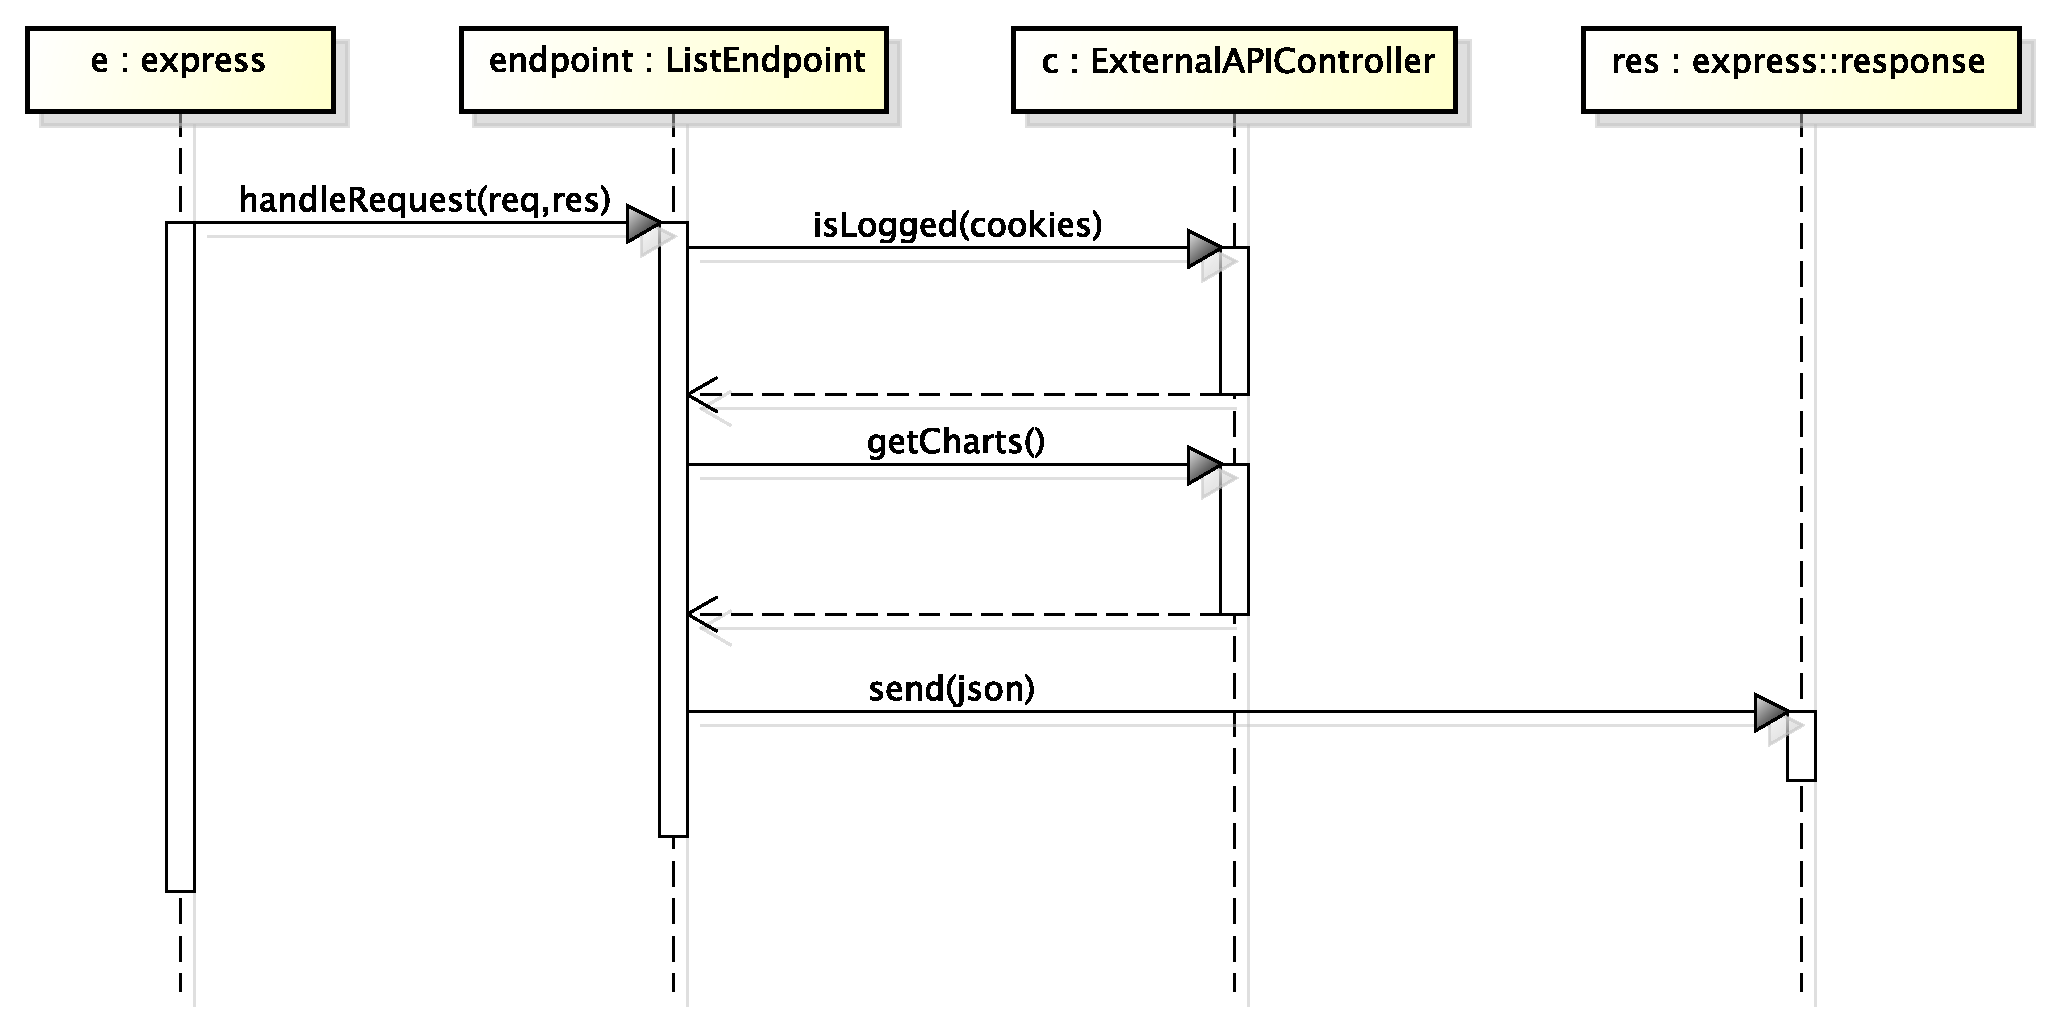
\includegraphics[scale=0.3]{DefinizioneDiProdotto/Pics/NorrisInvioLista}
                \caption{Diagramma di sequenza - Norris, invio lista}
            \end{figure}

            
        \level{3}{Invio di un chart}
        	Tale diagramma descrive come viene gestita la richiesta di un chart da parte di un \insglo{client} dal sistema \insglo{Norris}.
            \begin{figure}[H]
                \centering
                \includegraphics[scale=0.3]{DefinizioneDiProdotto/Pics/NorrisInvioChart}
                \caption{Diagramma di sequenza - Norris, invio chart}
            \end{figure}


    \level{3}{Classi aggiuntive}
        Per quanto riguarda le classi aggiuntive riguardanti che implementano i tipi “ChartSettings” e “ChartUpdate” si faccia riferimento all'appendice \nameref{app:schemi}, nella quale sono presenti gli schemi \insglo{JSON} di tali oggetti.
        
			\level{4}[NorrisSettingsImpl]{NorrisAggiuntive::NorrisSettingsImpl}
			

		\IfFileExists{DefinizioneDiProdotto/Pics/ClassiAggiuntive/NorrisSettingsImpl.pdf}{
			\begin{figure}[H]
				\centering
				\includegraphics[scale=0.5]{DefinizioneDiProdotto/Pics/ClassiAggiuntive/NorrisSettingsImpl}
				\caption{NorrisSettingsImpl}
			\end{figure}
		}
	
			
			\begin{itemize}
			\item \textbf{Nome:} NorrisSettingsImpl
			\item \textbf{Tipo:} classe
			
		\item \textbf{Astratta:}
		no
			\item \textbf{Visibilità:} public
			\item \textbf{Descrizione:} La classe NorrisSettingsImpl definisce le impostazioni relative ad un'istanza di Norris. Lo sviluppatore può definire le funzioni che verranno eseguite per l'autenticazione.
			\item \textbf{Attributi:}
				\begin{itemize}
				\setlength{\itemsep}{5pt}
				
					\item[\ding{111}] {+login : Function} \\ [1mm] L'attributo login rappresenta la funzione che verrà eseguita per avviare la sessione di un utente.
					\item[\ding{111}] {+logout : Function} \\ [1mm] L'attributo login rappresenta la funzione che verrà eseguita per terminare la sessione di un utente.
					\item[\ding{111}] {+keepAlive : Function} \\ [1mm] L'attributo login rappresenta la funzione che verrà eseguita per rinnovare la sessione di un utente.
					\item[\ding{111}] {+isLogged : Function} \\ [1mm] L'attributo login rappresenta la funzione che verrà eseguita per verificare lo stato dela sessione di un utente.
					\item[\ding{111}] {+endpoint : String} \\ [1mm] L'attributo endpoint definisce il path al quale sono disponibili le API esterne.
					\item[\ding{111}] {+secret : String} \\ [1mm] L'attributo secret definisce la chiave di cifrature per i cookie firmati.
					\item[\ding{111}] {+origins : String[]} \\ [1mm] L'attributo origin definisce gli host attendibili, verso i quali saranno disponibili le API esterne.
				\end{itemize}
		
			\end{itemize}
	
			\level{4}[PageSettingsImpl]{NorrisAggiuntive::PageSettingsImpl}
			

		\IfFileExists{DefinizioneDiProdotto/Pics/ClassiAggiuntive/PageSettingsImpl.pdf}{
			\begin{figure}[H]
				\centering
				\includegraphics[scale=0.5]{DefinizioneDiProdotto/Pics/ClassiAggiuntive/PageSettingsImpl}
				\caption{PageSettingsImpl}
			\end{figure}
		}
	
			
			\begin{itemize}
			\item \textbf{Nome:} PageSettingsImpl
			\item \textbf{Tipo:} classe
			
		\item \textbf{Astratta:}
		no
			\item \textbf{Visibilità:} public
			\item \textbf{Descrizione:} La classe PageSettingsImpl definisce le impostazioni di una pagina di Norris.
			\item \textbf{Attributi:}
				\begin{itemize}
				\setlength{\itemsep}{5pt}
				
					\item[\ding{111}] {+title : String} \\ [1mm] L'attributo title rappresenta il titolo di una pagina di Norris.
					\item[\ding{111}] {+maxChartsRow : int} \\ [1mm] L'attributo title rappresenta il numero massimo di righe visualizzabili all'interno della pagina.
					\item[\ding{111}] {+maxChartsCol : int} \\ [1mm] L'attributo title rappresenta il numero massimo di colonne visualizzabili all'interno della pagina.
				\end{itemize}
		
			\end{itemize}
	

    \level{2}{Diagrammi di sequenza}
    	In tale sezione vengono presentati i diagrammi di sequenza, che hanno lo scopo di descrivere scenari (determinate sequenze di azioni in cui tutte le scelte sono già state effettuate). Essi vengono usati per descrivere le relazioni che intercorrono, in termini di messaggi, tra attori, oggetti ed entità del sistema \insglo{Norris}.
        \level{3}{Creazione di un chart}
        	Tale diagramma descrive come viene creato un chart di un certo tipo prefissato.
            \begin{figure}[H]
                \centering
                \includegraphics[scale=0.3]{DefinizioneDiProdotto/Pics/NorrisCreazioneChart}
                \caption{Diagramma di sequenza - Norris, creazione chart}
            \end{figure}


        \level{3}{Aggiornamento di un chart}
        	Tale diagramma descrive come viene aggiornato un chart di un certo tipo (sulla base delle modalità di aggiornamento definite per quel tipo di grafico).
            \begin{figure}[H]
                \centering
                \includegraphics[scale=0.3]{DefinizioneDiProdotto/Pics/NorrisAggiornamentoChart}
                \caption{Diagramma di sequenza - Norris, aggiornamento chart}
            \end{figure}

            
        \level{3}{Invio lista dei grafici}
        	Tale diagramma descrive come viene gestita la richiesta della lista di tutti i grafici contenuti in una certa istanza di \insglo{Norris}.
            \begin{figure}[H]
                \centering
                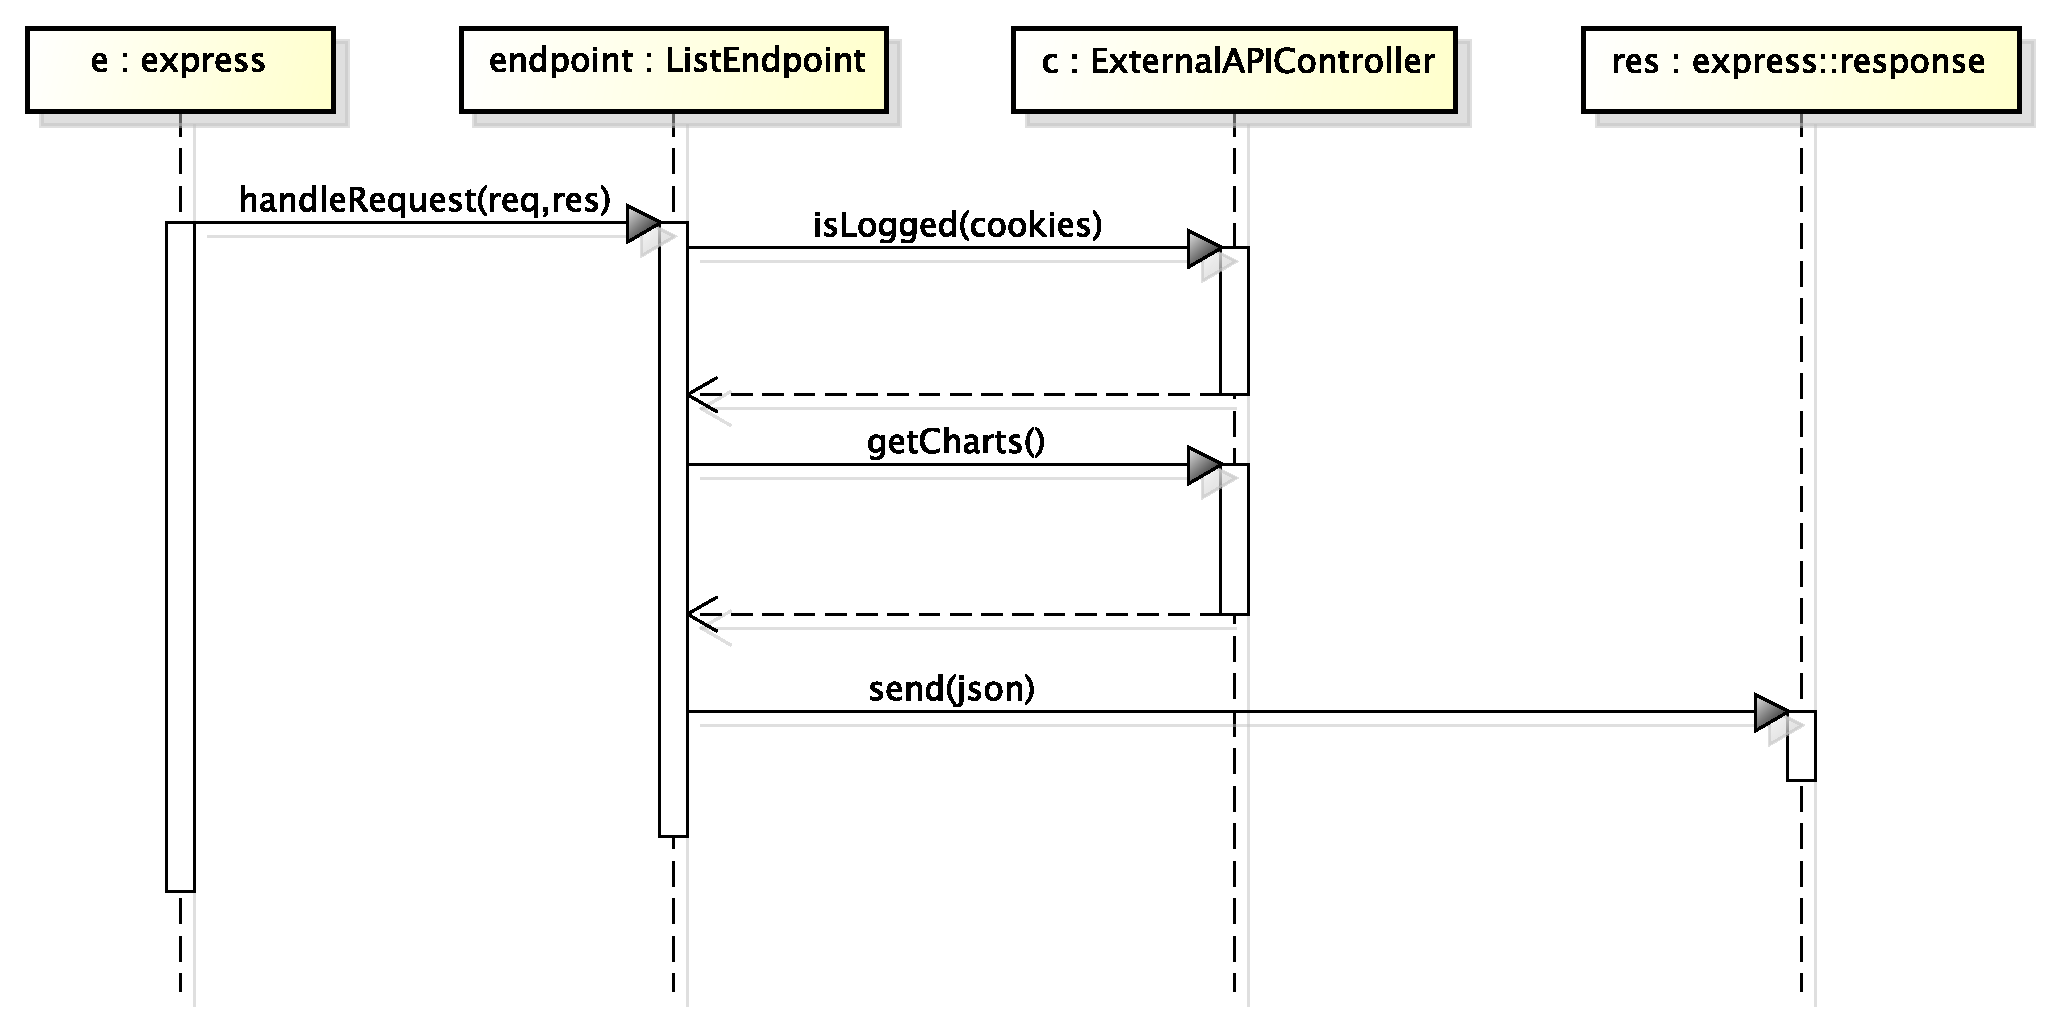
\includegraphics[scale=0.3]{DefinizioneDiProdotto/Pics/NorrisInvioLista}
                \caption{Diagramma di sequenza - Norris, invio lista}
            \end{figure}

            
        \level{3}{Invio di un chart}
        	Tale diagramma descrive come viene gestita la richiesta di un chart da parte di un \insglo{client} dal sistema \insglo{Norris}.
            \begin{figure}[H]
                \centering
                \includegraphics[scale=0.3]{DefinizioneDiProdotto/Pics/NorrisInvioChart}
                \caption{Diagramma di sequenza - Norris, invio chart}
            \end{figure}


    \level{3}{Classi aggiuntive}
        Per quanto riguarda le classi aggiuntive riguardanti che implementano i tipi “ChartSettings” e “ChartUpdate” si faccia riferimento all'appendice \nameref{app:schemi}, nella quale sono presenti gli schemi \insglo{JSON} di tali oggetti.
        
			\level{4}[NorrisSettingsImpl]{NorrisAggiuntive::NorrisSettingsImpl}
			

		\IfFileExists{DefinizioneDiProdotto/Pics/ClassiAggiuntive/NorrisSettingsImpl.pdf}{
			\begin{figure}[H]
				\centering
				\includegraphics[scale=0.5]{DefinizioneDiProdotto/Pics/ClassiAggiuntive/NorrisSettingsImpl}
				\caption{NorrisSettingsImpl}
			\end{figure}
		}
	
			
			\begin{itemize}
			\item \textbf{Nome:} NorrisSettingsImpl
			\item \textbf{Tipo:} classe
			
		\item \textbf{Astratta:}
		no
			\item \textbf{Visibilità:} public
			\item \textbf{Descrizione:} La classe NorrisSettingsImpl definisce le impostazioni relative ad un'istanza di Norris. Lo sviluppatore può definire le funzioni che verranno eseguite per l'autenticazione.
			\item \textbf{Attributi:}
				\begin{itemize}
				\setlength{\itemsep}{5pt}
				
					\item[\ding{111}] {+login : Function} \\ [1mm] L'attributo login rappresenta la funzione che verrà eseguita per avviare la sessione di un utente.
					\item[\ding{111}] {+logout : Function} \\ [1mm] L'attributo login rappresenta la funzione che verrà eseguita per terminare la sessione di un utente.
					\item[\ding{111}] {+keepAlive : Function} \\ [1mm] L'attributo login rappresenta la funzione che verrà eseguita per rinnovare la sessione di un utente.
					\item[\ding{111}] {+isLogged : Function} \\ [1mm] L'attributo login rappresenta la funzione che verrà eseguita per verificare lo stato dela sessione di un utente.
					\item[\ding{111}] {+endpoint : String} \\ [1mm] L'attributo endpoint definisce il path al quale sono disponibili le API esterne.
					\item[\ding{111}] {+secret : String} \\ [1mm] L'attributo secret definisce la chiave di cifrature per i cookie firmati.
					\item[\ding{111}] {+origins : String[]} \\ [1mm] L'attributo origin definisce gli host attendibili, verso i quali saranno disponibili le API esterne.
				\end{itemize}
		
			\end{itemize}
	
			\level{4}[PageSettingsImpl]{NorrisAggiuntive::PageSettingsImpl}
			

		\IfFileExists{DefinizioneDiProdotto/Pics/ClassiAggiuntive/PageSettingsImpl.pdf}{
			\begin{figure}[H]
				\centering
				\includegraphics[scale=0.5]{DefinizioneDiProdotto/Pics/ClassiAggiuntive/PageSettingsImpl}
				\caption{PageSettingsImpl}
			\end{figure}
		}
	
			
			\begin{itemize}
			\item \textbf{Nome:} PageSettingsImpl
			\item \textbf{Tipo:} classe
			
		\item \textbf{Astratta:}
		no
			\item \textbf{Visibilità:} public
			\item \textbf{Descrizione:} La classe PageSettingsImpl definisce le impostazioni di una pagina di Norris.
			\item \textbf{Attributi:}
				\begin{itemize}
				\setlength{\itemsep}{5pt}
				
					\item[\ding{111}] {+title : String} \\ [1mm] L'attributo title rappresenta il titolo di una pagina di Norris.
					\item[\ding{111}] {+maxChartsRow : int} \\ [1mm] L'attributo title rappresenta il numero massimo di righe visualizzabili all'interno della pagina.
					\item[\ding{111}] {+maxChartsCol : int} \\ [1mm] L'attributo title rappresenta il numero massimo di colonne visualizzabili all'interno della pagina.
				\end{itemize}
		
			\end{itemize}
	

    \level{2}{Diagrammi di sequenza}
    	In tale sezione vengono presentati i diagrammi di sequenza, che hanno lo scopo di descrivere scenari (determinate sequenze di azioni in cui tutte le scelte sono già state effettuate). Essi vengono usati per descrivere le relazioni che intercorrono, in termini di messaggi, tra attori, oggetti ed entità del sistema \insglo{Norris}.
        \level{3}{Creazione di un chart}
        	Tale diagramma descrive come viene creato un chart di un certo tipo prefissato.
            \begin{figure}[H]
                \centering
                \includegraphics[scale=0.3]{DefinizioneDiProdotto/Pics/NorrisCreazioneChart}
                \caption{Diagramma di sequenza - Norris, creazione chart}
            \end{figure}


        \level{3}{Aggiornamento di un chart}
        	Tale diagramma descrive come viene aggiornato un chart di un certo tipo (sulla base delle modalità di aggiornamento definite per quel tipo di grafico).
            \begin{figure}[H]
                \centering
                \includegraphics[scale=0.3]{DefinizioneDiProdotto/Pics/NorrisAggiornamentoChart}
                \caption{Diagramma di sequenza - Norris, aggiornamento chart}
            \end{figure}

            
        \level{3}{Invio lista dei grafici}
        	Tale diagramma descrive come viene gestita la richiesta della lista di tutti i grafici contenuti in una certa istanza di \insglo{Norris}.
            \begin{figure}[H]
                \centering
                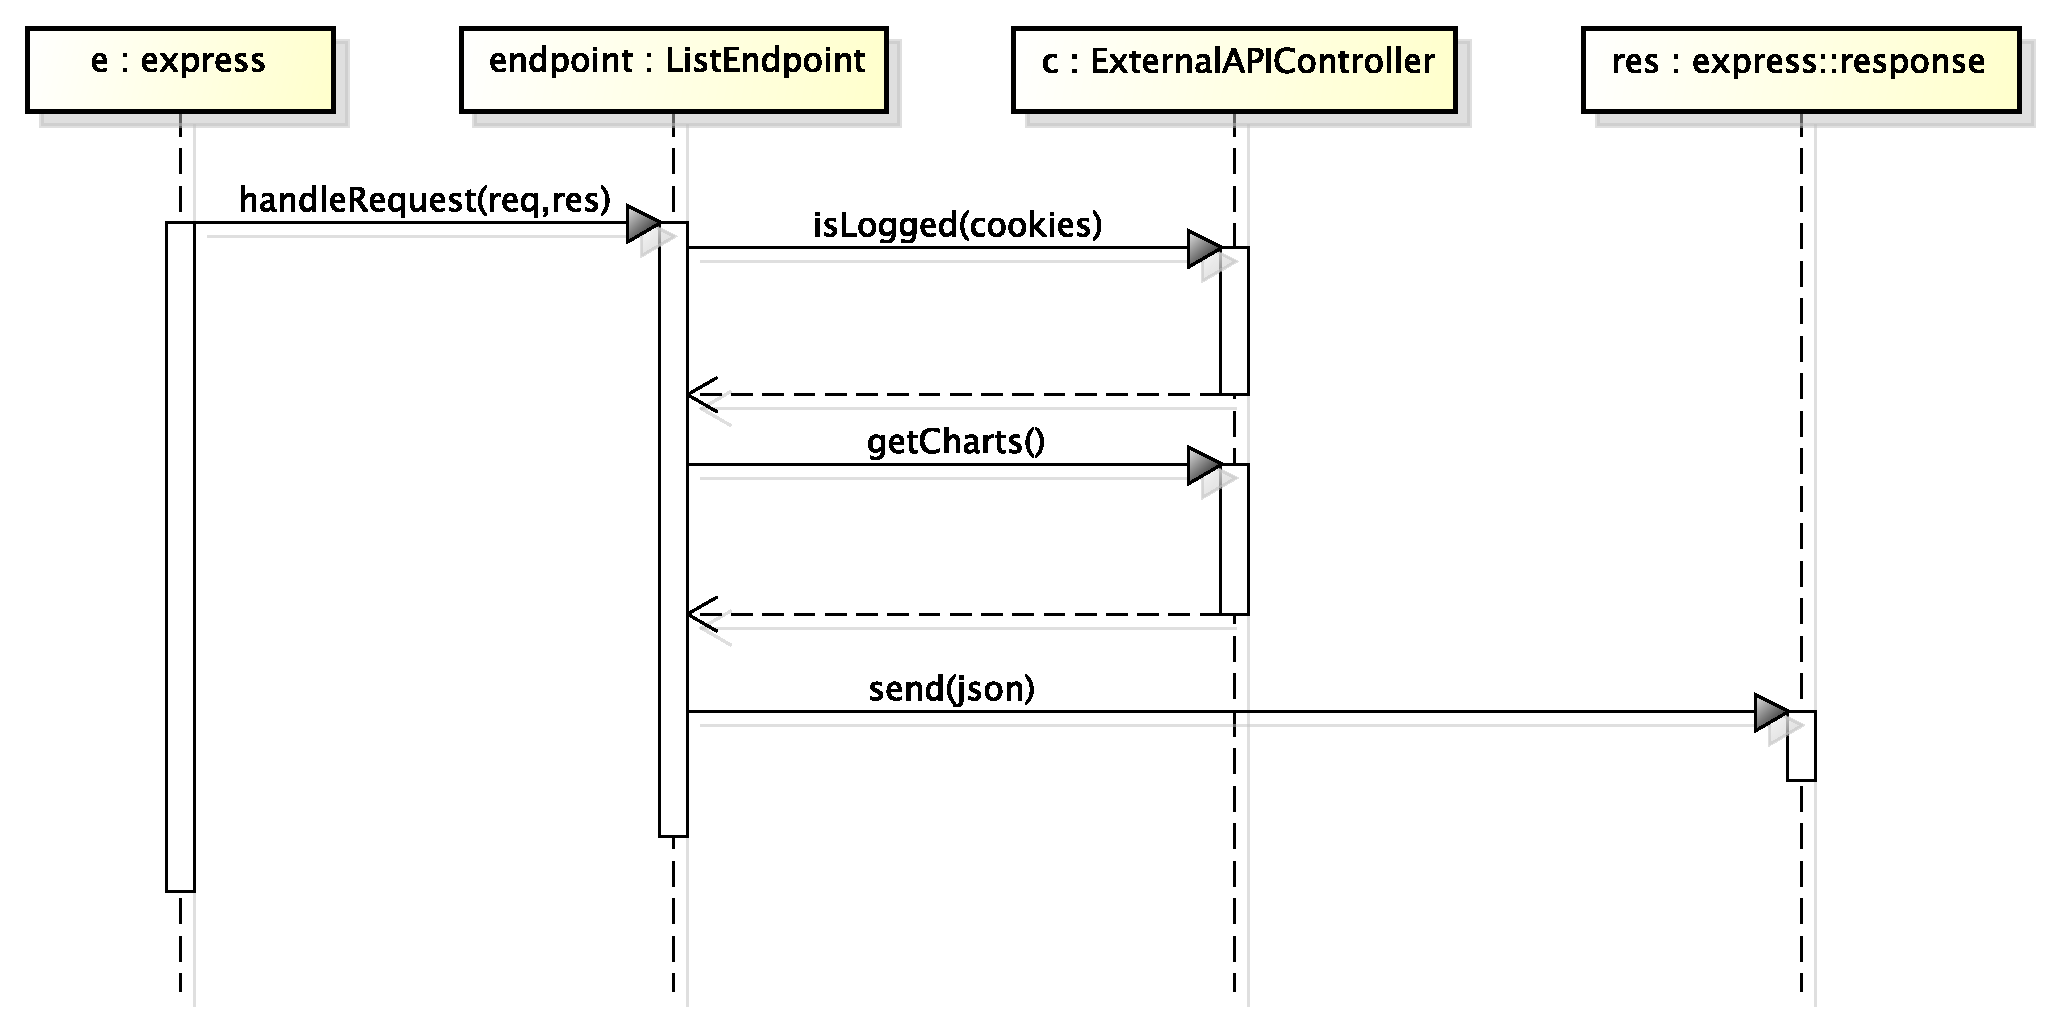
\includegraphics[scale=0.3]{DefinizioneDiProdotto/Pics/NorrisInvioLista}
                \caption{Diagramma di sequenza - Norris, invio lista}
            \end{figure}

            
        \level{3}{Invio di un chart}
        	Tale diagramma descrive come viene gestita la richiesta di un chart da parte di un \insglo{client} dal sistema \insglo{Norris}.
            \begin{figure}[H]
                \centering
                \includegraphics[scale=0.3]{DefinizioneDiProdotto/Pics/NorrisInvioChart}
                \caption{Diagramma di sequenza - Norris, invio chart}
            \end{figure}

	
		\newpage
		\level{2}{Chuck}
	\begin{figure}[H]\centering
        \includegraphics[width=\textwidth]{SpecificaTecnica/Pics/componentiChuck}
        \caption{Diagramma delle componenti di Chuck}
    \end{figure}
	\level{3}{Design Pattern utilizzati}
	Nella progettazione delle componenti di Chuck abbiamo deciso di utilizzare il design pattern MVC.
	MOTIVAZIONE
    \level{3}{Descrizione dei componenti di Chuck}
    	\level{4}{Chuck API Manager}
    		La componente Chuck Api Manager si occupa di implementare le funzionalità offerte dalle API di Chuck allo sviluppatore client. Queste funzionalità sono:
    		\begin{itemize}
						\item inserimento di nuovi grafici in un sito web;
						\item scelta del tag HTML in cui inserire un grafico;
						\item modifica di alcune impostazioni dei grafici;
						\item login;
						\item logout.
			\end{itemize}
    		Questa componente si occupa inoltre di gestire la comunicazione con Norris.
    		
    	\level{4}{Chart View}
    	La componente Chart View ha il compito di visualizzare i grafici all'interno della pagina web. I grafici possono essere del tipo Bar Chart, Line Chart, Map Chart e Table. Quando un grafico viene aggiornato, questa componente si occupa di aggiornare anche la sua visualizzazione nella pagina web.

    	\level{4}{Controller}
    	La componente Controller ha lo scopo di ricevere gli input provenienti dalla Chart View ed effettuarne la gestione. L'input consiste in un sottoinsieme di dataset scelti dall'utente che sta visualizzando la pagina web. Il Controller deve far sì che vengano visualizzati solo questi dataset, in modo da permettere all'utente di applicare un filtro sulle serie.

    	\level{4}{Data Model}
    	La componente Data Model è un modello che astrae i grafici visualizzati nella pagina web. In essa sono contenuti i dati riguardanti i grafici, assieme alle relative impostazioni. In particolare sono presenti i modelli di tutte le tipologie di chart implementati da Norris. Il Data Model fornisce per ciascuna tipologia di grafico i metodi per inserire i dati e configurare alcune impostazioni. 
    
	\level{3}{Descrizione delle interazioni tra le componenti}
	
		\level{4}{Chuck API Manager - Data Model}
		Quando il Web Developer utilizza le API di Chuck oppure quando arriva un messaggio da Norris, Chuck API Manager apporta le opportune modifiche al Data Model, in modo che quest'ultimo rispecchi costantemente lo stato dei grafici da visualizzare.

		\level{4}{Chart View - Data Model}
		Quando la Chart View deve aggiornare la visualizzazione del grafico, essa effettua una query sul Data Model per ottenere le nuove informazioni relative al grafico da aggiornare.

		\level{4}{Data Model - Chart View}
		Quando avviene una modifica nel Data Model, una notifica avvisa la Chart View dell'avvenuto cambiamento. In particolare ciò accade quando è stato inserito un nuovo grafico o quando è arrivato l'aggiornamento di un grafico già presente.

		\level{4}{Chart View - Controller}
		Quando la Chart View riceve un input dall'utente, una notifica avvisa il Controller in modo che intraprenda l'azione per gestirla.

		\level{4}{Controller - Chart View}
		In caso di necessità il controller può selezionare la Chart View da visualizzare.
		\level{4}{Controller - Data Model}
		Quando intraprende un'azione, il controller può effettuare delle modifiche nel Data Model. In particolare ciò accade quando si deve inserire un nuovo grafico o quando arriva l'aggiornamento di un grafico già presente.

	
		\newpage
		\level{1}{Applicazione}

	\level{2}{Classi}
		\level{1}{Applicazione}

	\level{2}{Classi}
		\level{1}{Applicazione}

	\level{2}{Classi}
		\input{Classi/Applicazione.tex}
	
		\newpage
		\level{2}{Dashboard APS}
	La \insglo{dashboard} è un esempio d'uso di \insglo{Norris}: rappresenta un modo in cui il \insglo{prodotto} può essere utilizzato. Essa, dunque, è una pagina web generata in automatico dal \insglo{server} \insglo{Norris}. Essa è costituita da più grafici che l'utente finale potrà visualizzare sul proprio \insglo{browser}. Di seguito viene fornito un \insglo{mockup} della pagina, che mostra a grandi linee come sarà visualizzata la \insglo{dashboard} una volta completata..
	\begin{figure}[H]\centering
        \includegraphics[width=\textwidth]{SpecificaTecnica/Pics/DashboardMockup}
        \caption{Mockup della dashboard APS}
    \end{figure}
    Vengono ora descritti i vari componenti di cui è fatta la pagina, ovvero vengono descritti i grafici che sono stati inseriti all'interno del \insglo{mockup} mostrato in precedenza.
    \level{3}{Descrizione delle componenti della Dashboard}
    	\level{4}{Map chart}
    		Tramite questo grafico l'utilizzatore della \insglo{dashboard} è in grado di visualizzare in tempo reale la posizione di tutti i bus attivi nelle varie linee dell'\insglo{APS}. Tale grafico mette inoltre a disposizione dell'utente delle opzioni riguardanti il filtraggio delle linee presenti: infatti, esso permette di scegliere le linee che si intendono visualizzare, semplicemente nascondendo e ignorando le rimanenti. In questo modo si può trasformare un grafico potenzialmente caotico (a causa della grande quantità di punti presenti al suo interno) in un molto più comprensibile e consultabile.
    	\level{4}{Table}
    		Tale grafico è dedicato ai punti di maggior interesse di Padova. Esso fornisce all'utente utilizzatore della \insglo{dashboard} il tempo necessario all'arrivo degli autobus in alcune fermate \insglo{APS} molto frequentate. In particolare, è possibile visualizzare quanto tempo manca all'arrivo del prossimo autobus in una determinata stazione, e a quale linea il suddetto autobus appartiene. Grazie ad esso gli utenti sono in grado di capire quanto devono attendere mediamente prima di poter salire su uno dei mezzi da loro scelti.
    	\level{4}{Bar chart}
    		Questo grafico permette all'utilizzatore della \insglo{dashboard} di visualizzare quanti autobus sono attivi su ciascuna linea dell'\insglo{APS}. Tale grafico mette inoltre a disposizione dell'utente delle opzioni riguardanti il filtraggio delle linee presenti: infatti, esso permette di scegliere le linee di cui si vuole visualizzare il numero di bus attivi. Grazie a questo grafico, l'utente può ottenere utili informazioni su quanto una linea è frequentata e sul tempo di attesa che mediamente passa tra làarrivo di un mezzo e del successivo.
    \level{3}{Creazione della Dashboard}
        In questa sezione viene mostrato quali sono i passi principali che l'utilizzatore di \insglo{Norris} deve fare per creare la \insglo{Dashboard} \insglo{APS}. La descrizione che segue può essere maggiormente compresa grazie al diagramma delle attività qui presente.
        \begin{figure}[H]\centering
            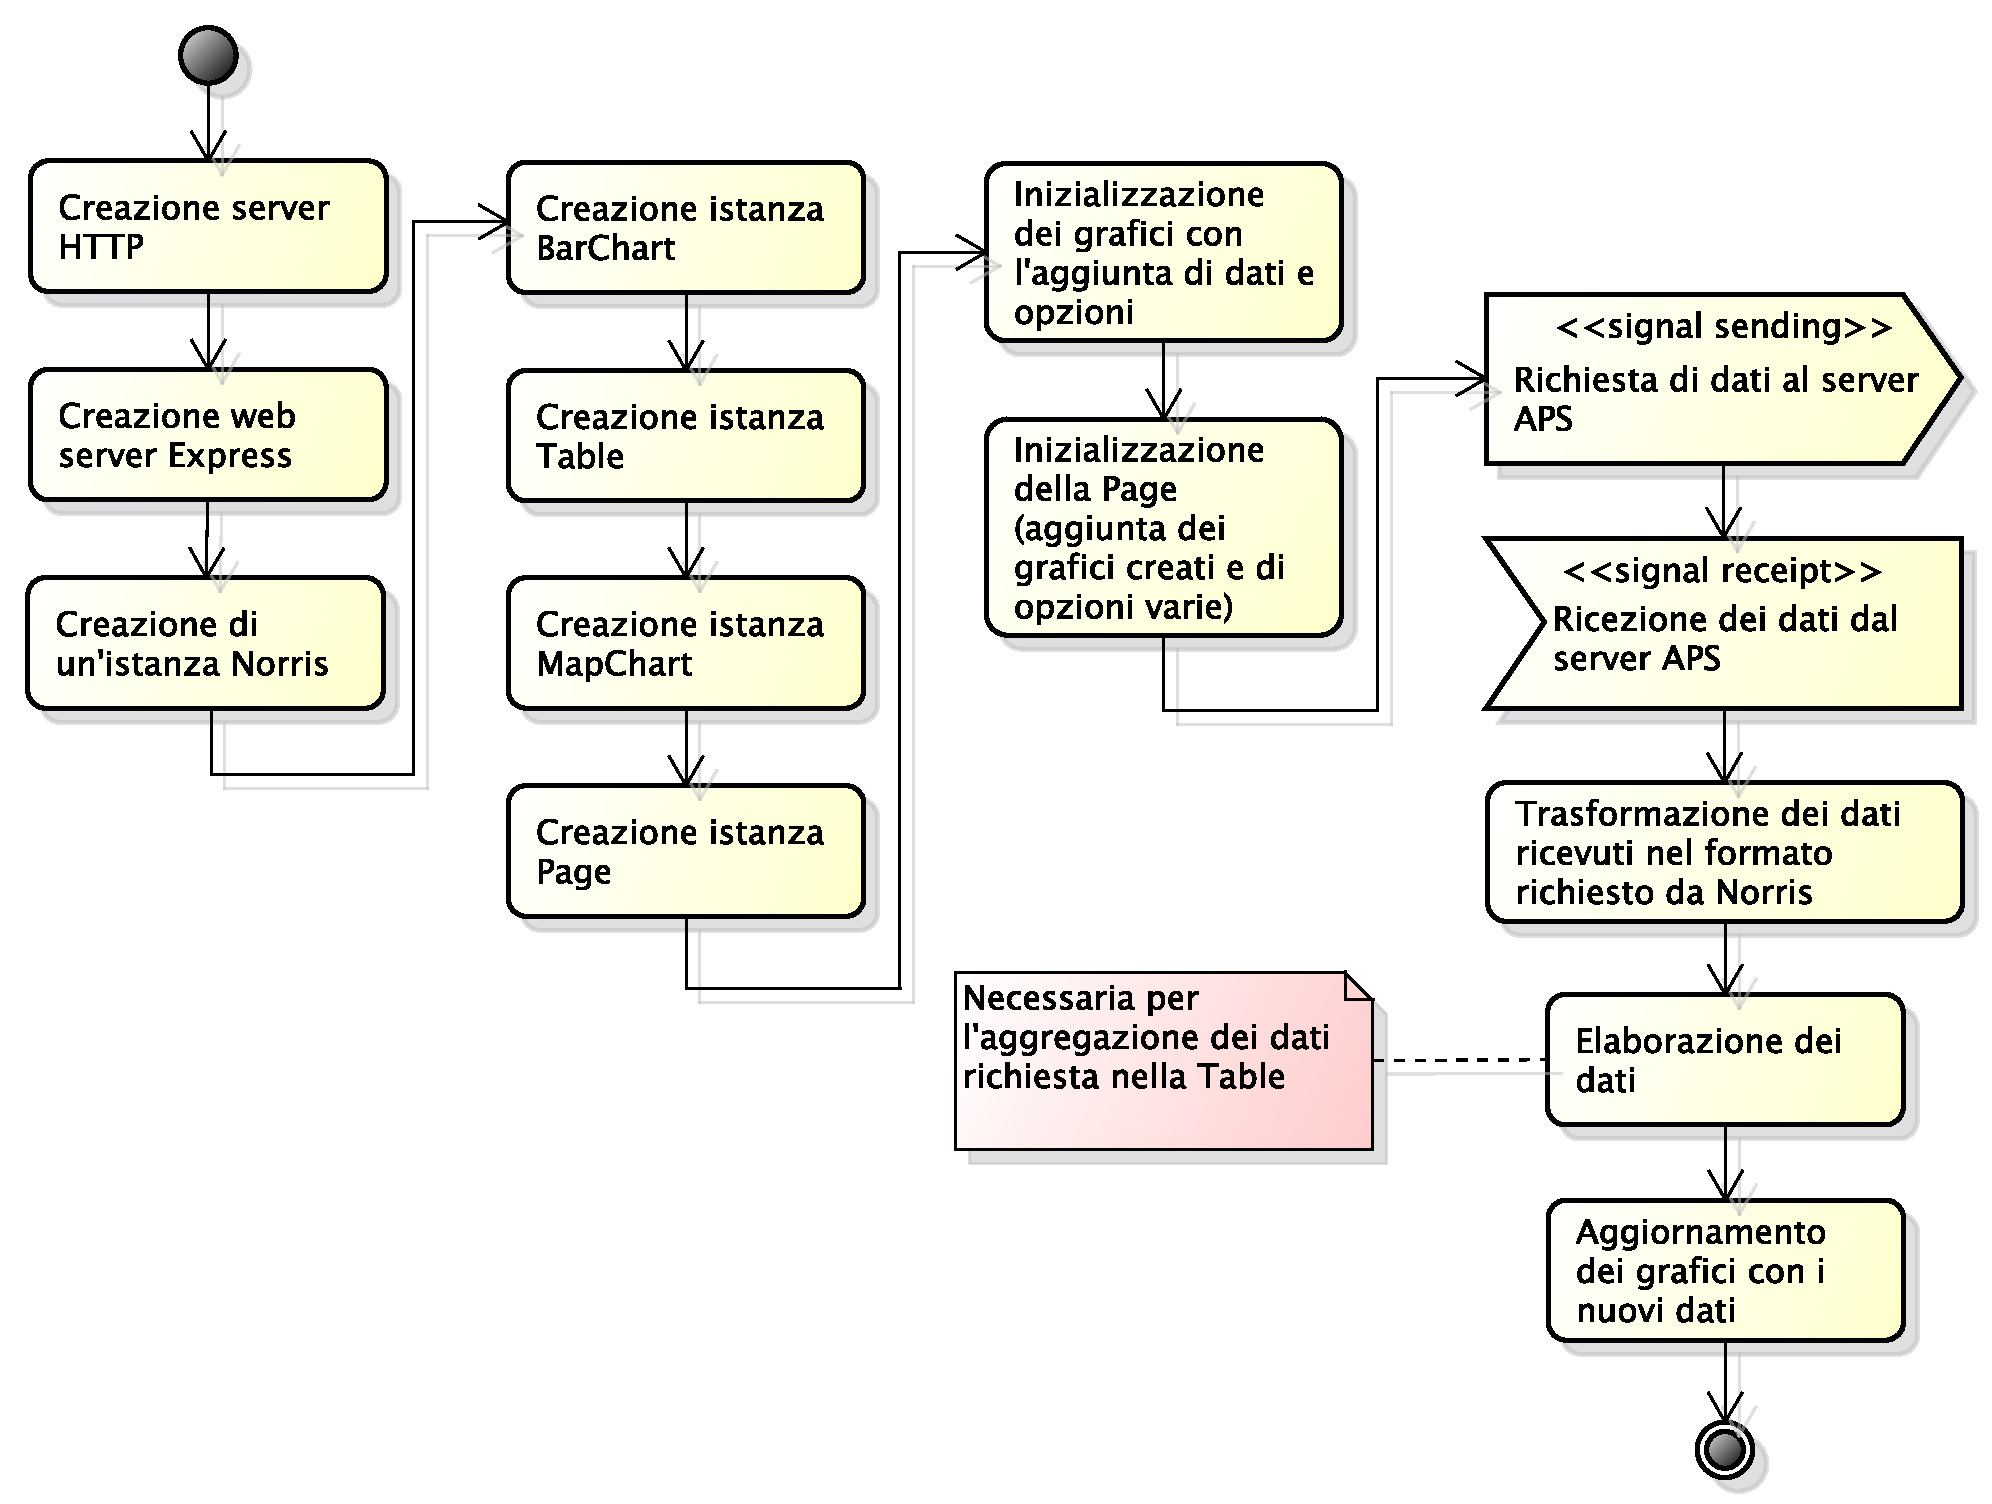
\includegraphics[width=\textwidth]{SpecificaTecnica/Pics/CreateDashboard}
            \caption{Creazione della Dashboard - diagramma delle attività}
        \end{figure}
        \begin{enumerate}
            \item Requisito fondamentale per la creazione della \insglo{dashboard} è che esista e sia correttamente funzionante un'istanza di \insglo{Norris}. Dunque, seppur banale, la prima cosa che l'utilizzatore di \insglo{Norris} deve fare è assicurarsi di ciò.
            \item In secondo luogo vanno creati i grafici che dovranno essere contenuti nella pagina web. Essi inizialmente sono vuoti (sono privi di impostazioni e di dati, che verranno aggiunti successivamente). Lo sviluppatore fa uso dell'interfaccia \texttt{\insglo{Norris}::InternalAPIManager::\insglo{Norris}} per fare ciò. Essa è presentata e descritta all'interno di questo documento (vedi progettazione architetturale di \insglo{Norris}).
            \item A questo punto va creata la pagina che dovrà contenere i grafici creati in precedenza. Inizialmente, dunque, anch'essa sarà vuota, ovvero priva di contenuto (i grafici) e di opzioni. Per creare la pagina va utilizzata ancora una volta l'interfaccia disponibile allo sviluppatore \texttt{\insglo{Norris}::InternalAPIManager::\insglo{Norris}} (vedi progettazione architetturale di \insglo{Norris}).
            \item Compito dello sviluppatore è ora quello di inizializzare i grafici creati in precedenza, mediante l'aggiunta di eventuali dati e impostazioni.
            \begin{itemize}
                \item Per quanto riguarda il BarChart e il MapChart essi saranno inizialmente vuoti. Infatti, i dati verranno aggiunti mano a mano che verranno ricevuti dai \insglo{server} dell'\insglo{APS}, in un momento successivo.\\
                Le impostazioni, invece, possono già essere scelte per entrambi i chart (per esempio il titolo, la descrizione, la posizione della legenda ecc.).\\
                Sia per inserire un insieme vuoto di dati iniziali, sia per impostare le opzioni dei grafici, si fa uso dell'interfaccia \texttt{\insglo{Norris}::InternalAPIManager::Chart}, descritta e documentata all'interno del presente documento (vedi progettazione architetturale \insglo{Norris}).
                \item La \insglo{Table}, invece, inizialmente non sarà del tutto vuota (seppur inutilizzabile). Infatti, nonostante non si conoscano ancora le posizioni dei vari mezzi dell'\insglo{APS}, si devono inserire i nomi dei punti di interesse che si vogliono monitorare successivamente. Ci si deve contemporaneamente preoccupare di rendere evidente il fatto che non siano ancora disponibili dati su cui basare i calcoli del tempo medio di attesa (per esempio impostando il valore “unknown” nei campi “Linea del prossimo bus in arrivo” e “tempo di attesa medio”).\\
                Per quanto riguarda le impostazioni, esse possono essere scelte liberamente dallo svilupparoe.\\
                Sia per inserire i dati iniziali, sia per impostare le opzioni del grafico, si fa uso dell'interfaccia \texttt{\insglo{Norris}::InternalAPIManager::Chart}, descritta e documentata all'interno del presente documento (vedi progettazione architetturale \insglo{Norris}).
            \end{itemize}
            \item Dopo aver inizializzato i grafici in modo corretto, lo sviluppatore li inserisce all'interno della pagina creata in precedenza. Egli può inoltre scegliere liberamente le impostazioni della pagina.\\
            Lo sviluppatore fa uso dell'interfaccia \texttt{\insglo{Norris}::InternalAPIManager::Page} per eseguire questi compiti. Tale interfaccia è presentata e descritta all'interno di questo documento (vedi progettazione architetturale di \insglo{Norris}).
            \item Ora che tutti i vari elementi sono stati correttamente inizializzati, allo sviluppatore non resta che tenere costantemente aggiornati i dati contenuti all'interno dei grafici (e dunque della pagina). Per fare ciò, egli deve innanzitutto preoccuparsi di richiedere i dati riguardanti le varie linee al \insglo{server} dell'\insglo{APS}.
            \item Una volta ottenuti i dati, lo sviluppatore si deve preoccupare di convertirli in un formato fruibile da \insglo{Norris}. Essi, infatti, sono nel formato fornito dall'\insglo{APS}, che non necessariamente è lo stesso di quello utilizzato dai nostri prodotti.
            \item I dati a questo punto vanno aggregati e/o elaborati nel modo richiesto dai vari grafici presenti.
            \begin{itemize}
                \item Per la \insglo{Table} si devono utilizzare i dati a disposizione per capire il mezzo più vicino a un dato punto e per calcolare il tempo medio di attesa.
                \item Per il \insglo{Bar Chart} si devono utilizzare i dati a disposizione per calcolare quanti mezzi sono attivi al momento per ciascuna linea presente.
            \end{itemize}
            \item Infine, grazie ai dati ottenuti e ai calcoli eseguiti precedentemente, lo sviluppatore è in grado di aggiornare i vari grafici. Gli aggiornamenti avvengono in base alla tipologia di grafico e in base ai risultati che sono stati ottenuti precedentemente.\\
            Prima di cominciare un nuovo processo di aggiornamento (tramite la richiesta di dati al \insglo{server} \insglo{APS}), si attende per un tempo prefissato (minore è il tempo di aggiornamento, maggiore sarà la reattività e la precisione della \insglo{Dashboard}).
        \end{enumerate}
	
		\newpage
		\level{1}{Tracciamento}
	\level{2}{Componenti-Requisiti}
	
				\begin{longtabu} spread 1cm [c]{|X[l]|X[l]|X[l]|}
					\hline
					\rowfont{\bf \centering}
					Codice &
					Dettaglio &
					Requisiti abbinati \\
					\hline
					\endhead
					
					N001 & Norris::InternalAPIManager & \parbox[t]{4cm}{ RRF1 \\ RRF1.1 \\ RRF1.2 \\ RRF1.3 \\ RRF1.4 \\ RRF1.5 \\ RRF1.5.1 \\ RRF1.5.1.1 \\ RRF1.5.1.2 \\ RRF1.5.2 \\ RRF1.5.2.2 \\ RRF1.5.3 \\ RRF1.5.3.1 \\ RRF1.5.3.2 \\ RDF1.5.4 \\ RRF1.5.5 \\ RRF1.5.5.1 \\ RRF1.5.5.2 \\ RRF1.5.6 \\ RRF1.5.6.1 \\ RRF1.5.6.2 \\ RRF1.5.7 \\ RRF1.5.7.1 \\ RRF1.5.7.2 \\ RDF1.5.7.3 \\ RRF1.5.7.4 \\ RDF1.5.7.5 \\ RDF1.5.7.6 \\ RRF1.5.7.7 \\ RRF1.5.8 \\ RRF1.5.9 \\ RRF1.5.10 \\ RRF1.5.11 \\ RRF1.5.12 \\ RRF1.5.13 \\ RRF1.5.14 \\ RRF1.5.15 \\ RRF1.5.16 \\ RRF1.5.17 \\ RRF1.5.18 \\ RRF1.5.18 \\ RRF1.5.19 \\ RRF1.5.20 \\ RRF1.5.21 \\ RRF1.5.22 \\ RRF1.5.23 \\ RRF1.6 \\ RRF1.7 \\ RRF1.8} \\ \hline
                                        N001 & Norris::InternalAPIManager & \parbox[t]{4cm}{ RRF1.9 \\ RRF1.10 \\ RRF2 \\ RRF2.1 \\ RRF2.2 \\ RRF2.3 \\ RRF2.4 \\ RRF2.5 \\ RRF2.6 \\ RRF3 \\ RRF2.7 \\ RRF3.1 \\ RRF3.2 \\ RRF3.2.1 \\ RRF3.2.2 \\ RRF3.3 \\ RRF4 \\ RRC10 \\ RRF1.5.2.1 }\\
                \hline
                N002 & Norris::ExternalAPIManager & \parbox[t]{4cm}{ RRF5 \\ RRF5.1 \\ RRF5.1.1 \\ RRF5.3 \\ RRF5.4 \\ RRC10 \\ RRC11 \\ RRF9 \\ RRF6.4 \\ RRF6.3 \\ RRF8.3 }\\
                \hline
                N003 & Norris::DataModel & \parbox[t]{4cm}{ RRF1.4 \\ RRF1 \\ RRF1.1 \\ RRF1.2 \\ RRF1.3 \\ RRF1.5 \\ RRF1.5.1 \\ RRF1.5.1.1 \\ RRF1.5.1.2 \\ RRF1.5.2 \\ RRF1.5.2.2 \\ RRF1.5.3 \\ RRF1.5.3.1 \\ RRF1.5.3.2 \\ RDF1.5.4 \\ RRF1.5.5 \\ RRF1.5.5.1 \\ RRF1.5.5.2 \\ RRF1.5.6 \\ RRF1.5.6.1 \\ RRF1.5.6.2} \\ \hline 
                N003 & Norris::DataModel & \parbox[t]{4cm}{ RRF1.5.7 \\ RRF1.5.7.1 \\ RRF1.5.7.2 \\ RDF1.5.7.3 \\ RRF1.5.7.4 \\ RDF1.5.7.5 \\ RDF1.5.7.6 \\ RRF1.5.7.7 \\ RRF1.5.8 \\ RRF1.5.9 \\ RRF1.5.10 \\ RRF1.5.11 \\ RRF1.5.12 \\ RRF1.5.13 \\ RRF1.5.14 \\ RRF1.5.15 \\ RRF1.5.16 \\ RRF1.5.17 \\ RRF1.5.18 \\ RRF1.5.19 \\ RRF1.5.20 \\ RRF1.5.21 \\ RRF1.5.22 \\ RRF1.5.23 \\ RRF1.6 \\ RRF1.7 \\ RRF1.9 \\ RRF1.8 \\ RRF1.10 \\ RRF2 \\ RRF2.1 \\ RRF2.2 \\ RRF2.3 \\ RRF2.4 \\ RRF2.5 \\ RRF2.6 \\ RRF3 \\ RRF2.7 \\ RRF3.1 \\ RRF3.2 \\ RRF3.2.1 \\ RRF3.2.2 \\ RRF3.3 \\ RRF5 \\ RRF5.1 \\ RRF5.1.1 \\ RRF5.2 \\ RRF1.5.2.1 \\ RRF6.4 }\\
                \hline
                C001 & Chuck::Directive & \parbox[t]{4cm}{ RRF6 \\ RRF6.1 \\ RDF6.2.1 \\ RDF6.2.2 \\ RDF6.2.3 \\ RDF6.2.4 \\ RDF6.2.5 \\ RDF6.2.6 \\ RDF6.2.7 \\ RDF6.2.8 \\ RDF6.2.9 \\ RDF6.2.10 \\ RDF6.2.11 \\ RDF6.2.12 \\ RDF6.2.13 }\\
                \hline
                C002 & Chuck::View & \parbox[t]{4cm}{ RRF6 \\ RDC18 }\\
                \hline
                C003 & Chuck::ViewModel & \parbox[t]{4cm}{ RRF6 \\ RDF6.2.1 \\ RDF6.2.2 \\ RDF6.2.3 \\ RDF6.2.4 \\ RDF6.2.5 \\ RDF6.2.6 \\ RDF6.2.7 \\ RDF6.2.8 \\ RDF6.2.9 \\ RDF6.2.10 \\ RDF6.2.11 \\ RDF6.2.12 \\ RDF6.2.13 }\\
                \hline
                C004 & Chuck::Model & \parbox[t]{4cm}{ RRF6 \\ RDF6.2.1 \\ RDF6.2.2 \\ RDF6.2.3 \\ RDF6.2.4 \\ RDF6.2.5 \\ RDF6.2.6 \\ RDF6.2.7 \\ RDF6.2.8 \\ RDF6.2.9 \\ RDF6.2.10 \\ RDF6.2.11 \\ RDF6.2.12 \\ RDF6.2.13 \\ RDF6.2 \\ RRF6.4 }\\
                \hline
                A001 & Applicazione::Model & \parbox[t]{4cm}{ ROF8 \\ RRF8.2 \\ RRF8.4 \\ RRF8.5 }\\
                \hline
                A002 & Applicazione::View & \parbox[t]{4cm}{ ROF8 \\ RRF8.1 \\ RRF8.2 \\ RRF8.4 \\ RRF8.5 }\\
                \hline
                A003 & Applicazione::Presenter & \parbox[t]{4cm}{ ROF8 \\ RRF8.1 \\ RRF8.2 \\ RRF8.4 \\ RRF8.5 }\\
                \hline
                A004 & Applicazione::Model::NorrisChart & \parbox[t]{4cm}{ ROF8 }\\
                \hline
                A005 & Applicazione::Model::Service & \parbox[t]{4cm}{ ROF8 \\ RRF8.3 }\\
                \hline
                N004 & Norris::DataModel::NorrisChart & \parbox[t]{4cm}{ RRF1.6 }\\
                \hline
                N005 & Norris::DataModel::NorrisPage & \parbox[t]{4cm}{ RRF3 }\\
                \hline
                C005 & Chuck::Model::NorrisChart & \parbox[t]{4cm}{ RRF1 \\ RRF1.1 \\ RRF1.2 \\ RRF1.3 \\ RRF1.4 \\ RRF2 \\ RRF2.1 \\ RRF2.2 \\ RRF2.3 \\ RRF2.4 \\ RRF2.5 \\ RRF2.6 \\ RRF2.7 }\\
                \hline
                C006 & Chuck::Model::Services & \parbox[t]{4cm}{ RRF6.3 \\ RRC17 }\\
                \hline
                                \caption{Tracciamento componenti-requisiti}
				\end{longtabu}
				
	\level{2}{Requisiti-Componenti}
	
				\begin{longtabu} spread 1cm [c]{|X[l]|X[l]|}
					\hline
					\rowfont{\bf \centering}
					Requisito &
					Componente \\
					\hline
					\endhead
					
					RRF1 & \parbox[t]{4cm}{ N001 \\ N003 \\ C005 } \\ 
                \hline
                RRF1.1 & \parbox[t]{4cm}{ N001 \\ N003 \\ C005 } \\ 
                \hline
                RRF1.5 & \parbox[t]{4cm}{ N001 \\ N003 } \\ 
                \hline
                RRF1.5.17 & \parbox[t]{4cm}{ N001 \\ N003 } \\ 
                \hline
                RRF1.5.1 & \parbox[t]{4cm}{ N001 \\ N003 } \\ 
                \hline
                RRF1.5.1.1 & \parbox[t]{4cm}{ N001 \\ N003 } \\ 
                \hline
                RRF1.5.1.2 & \parbox[t]{4cm}{ N001 \\ N003 } \\ 
                \hline
                RRF1.5.5 & \parbox[t]{4cm}{ N001 \\ N003 } \\ 
                \hline
                RRF1.5.5.1 & \parbox[t]{4cm}{ N001 \\ N003 } \\ 
                \hline
                RRF1.5.5.2 & \parbox[t]{4cm}{ N001 \\ N003 } \\ 
                \hline
                RDF1.5.4 & \parbox[t]{4cm}{ N001 \\ N003 } \\ 
                \hline
                RRF1.5.18 & \parbox[t]{4cm}{ N001 \\ N001 \\ N003 } \\ 
                \hline
                RRF1.5.7 & \parbox[t]{4cm}{ N001 \\ N003 } \\ 
                \hline
                RRF1.5.7.1 & \parbox[t]{4cm}{ N001 \\ N003 } \\ 
                \hline
                RRF1.5.7.2 & \parbox[t]{4cm}{ N001 \\ N003 } \\ 
                \hline
                RDF1.5.7.3 & \parbox[t]{4cm}{ N001 \\ N003 } \\ 
                \hline
                RRF1.5.7.4 & \parbox[t]{4cm}{ N001 \\ N003 } \\ 
                \hline
                RDF1.5.7.6 & \parbox[t]{4cm}{ N001 \\ N003 } \\ 
                \hline
                RRF1.5.7.7 & \parbox[t]{4cm}{ N001 \\ N003 } \\ 
                \hline
                RDF1.5.7.5 & \parbox[t]{4cm}{ N001 \\ N003 } \\ 
                \hline
                RRF1.5.8 & \parbox[t]{4cm}{ N001 \\ N003 } \\ 
                \hline
                RRF1.5.21 & \parbox[t]{4cm}{ N001 \\ N003 } \\ 
                \hline
                RRF1.5.9 & \parbox[t]{4cm}{ N001 \\ N003 } \\ 
                \hline
                RRF1.5.10 & \parbox[t]{4cm}{ N001 \\ N003 } \\ 
                \hline
                RRF1.5.11 & \parbox[t]{4cm}{ N001 \\ N003 } \\ 
                \hline
                RRF1.5.12 & \parbox[t]{4cm}{ N001 \\ N003 } \\ 
                \hline
                RRF1.5.13 & \parbox[t]{4cm}{ N001 \\ N003 } \\ 
                \hline
                RRF1.5.14 & \parbox[t]{4cm}{ N001 \\ N003 } \\ 
                \hline
                RRF1.5.15 & \parbox[t]{4cm}{ N001 \\ N003 } \\ 
                \hline
                RRF1.5.16 & \parbox[t]{4cm}{ N001 \\ N003 } \\ 
                \hline
                RRF1.5.2 & \parbox[t]{4cm}{ N001 \\ N003 } \\ 
                \hline
                RRF1.5.2.1 & \parbox[t]{4cm}{ N001 \\ N003 } \\ 
                \hline
                RRF1.5.2.2 & \parbox[t]{4cm}{ N001 \\ N003 } \\ 
                \hline
                RRF1.5.3 & \parbox[t]{4cm}{ N001 \\ N003 } \\ 
                \hline
                RRF1.5.3.1 & \parbox[t]{4cm}{ N001 \\ N003 } \\ 
                \hline
                RRF1.5.3.2 & \parbox[t]{4cm}{ N001 \\ N003 } \\ 
                \hline
                RRF1.5.6 & \parbox[t]{4cm}{ N001 \\ N003 } \\ 
                \hline
                RRF1.5.6.1 & \parbox[t]{4cm}{ N001 \\ N003 } \\ 
                \hline
                RRF1.5.6.2 & \parbox[t]{4cm}{ N001 \\ N003 } \\ 
                \hline
                RRF1.5.19 & \parbox[t]{4cm}{ N001 \\ N003 } \\ 
                \hline
                RRF1.5.20 & \parbox[t]{4cm}{ N001 \\ N003 } \\ 
                \hline
                RRF1.5.22 & \parbox[t]{4cm}{ N001 \\ N003 } \\ 
                \hline
                RRF1.5.23 & \parbox[t]{4cm}{ N001 \\ N003 } \\ 
                \hline
                RRF1.6 & \parbox[t]{4cm}{ N001 \\ N003 \\ N004 } \\ 
                \hline
                RRF1.2 & \parbox[t]{4cm}{ N001 \\ N003 \\ C005 } \\ 
                \hline
                RRF1.3 & \parbox[t]{4cm}{ N001 \\ N003 \\ C005 } \\ 
                \hline
                RRF1.4 & \parbox[t]{4cm}{ N001 \\ N003 \\ C005 } \\ 
                \hline
                RRF1.7 & \parbox[t]{4cm}{ N001 \\ N003 } \\ 
                \hline
                RRF1.8 & \parbox[t]{4cm}{ N001 \\ N003 } \\ 
                \hline
                RRF1.9 & \parbox[t]{4cm}{ N001 \\ N003 } \\ 
                \hline
                RRF1.10 & \parbox[t]{4cm}{ N001 \\ N003 } \\ 
                \hline
                RRF2 & \parbox[t]{4cm}{ N001 \\ N003 \\ C005 } \\ 
                \hline
                RRF2.1 & \parbox[t]{4cm}{ N001 \\ N003 \\ C005 } \\ 
                \hline
                RRF2.2 & \parbox[t]{4cm}{ N001 \\ N003 \\ C005 } \\ 
                \hline
                RRF2.3 & \parbox[t]{4cm}{ N001 \\ N003 \\ C005 } \\ 
                \hline
                RRF2.4 & \parbox[t]{4cm}{ N001 \\ N003 \\ C005 } \\ 
                \hline
                RRF2.5 & \parbox[t]{4cm}{ N001 \\ N003 \\ C005 } \\ 
                \hline
                RRF2.6 & \parbox[t]{4cm}{ N001 \\ N003 \\ C005 } \\ 
                \hline
                RRF2.7 & \parbox[t]{4cm}{ N001 \\ N003 \\ C005 } \\ 
                \hline
                RRF3 & \parbox[t]{4cm}{ N001 \\ N003 \\ N005 } \\ 
                \hline
                RRF3.1 & \parbox[t]{4cm}{ N001 \\ N003 } \\ 
                \hline
                RRF3.2 & \parbox[t]{4cm}{ N001 \\ N003 } \\ 
                \hline
                RRF3.2.1 & \parbox[t]{4cm}{ N001 \\ N003 } \\ 
                \hline
                RRF3.2.2 & \parbox[t]{4cm}{ N001 \\ N003 } \\ 
                \hline
                RRF3.3 & \parbox[t]{4cm}{ N001 \\ N003 } \\ 
                \hline
                RRF4 & \parbox[t]{4cm}{ N001 } \\ 
                \hline
                RRF5 & \parbox[t]{4cm}{ N002 \\ N003 } \\ 
                \hline
                RRF5.1 & \parbox[t]{4cm}{ N002 \\ N003 } \\ 
                \hline
                RRF5.1.1 & \parbox[t]{4cm}{ N002 \\ N003 } \\ 
                \hline
                RRF5.2 & \parbox[t]{4cm}{ N003 } \\ 
                \hline
                RRF5.3 & \parbox[t]{4cm}{ N002 } \\ 
                \hline
                RRF5.4 & \parbox[t]{4cm}{ N002 } \\ 
                \hline
                RRF6 & \parbox[t]{4cm}{ C001 \\ C004 \\ C003 \\ C002 } \\ 
                \hline
                RRF6.1 & \parbox[t]{4cm}{ C001 } \\ 
                \hline
                RDF6.2 & \parbox[t]{4cm}{ C004 } \\ 
                \hline
                RDF6.2.1 & \parbox[t]{4cm}{ C001 \\ C003 \\ C004 } \\ 
                \hline
                RDF6.2.4 & \parbox[t]{4cm}{ C001 \\ C003 \\ C004 } \\ 
                \hline
                RDF6.2.7 & \parbox[t]{4cm}{ C001 \\ C003 \\ C004 } \\ 
                \hline
                RDF6.2.9 & \parbox[t]{4cm}{ C001 \\ C003 \\ C004 } \\ 
                \hline
                RDF6.2.12 & \parbox[t]{4cm}{ C001 \\ C003 \\ C004 } \\ 
                \hline
                RDF6.2.13 & \parbox[t]{4cm}{ C001 \\ C003 \\ C004 } \\ 
                \hline
                RDF6.2.10 & \parbox[t]{4cm}{ C001 \\ C003 \\ C004 } \\ 
                \hline
                RDF6.2.11 & \parbox[t]{4cm}{ C001 \\ C003 \\ C004 } \\ 
                \hline
                RDF6.2.8 & \parbox[t]{4cm}{ C001 \\ C003 \\ C004 } \\ 
                \hline
                RDF6.2.5 & \parbox[t]{4cm}{ C001 \\ C003 \\ C004 } \\ 
                \hline
                RDF6.2.6 & \parbox[t]{4cm}{ C001 \\ C003 \\ C004 } \\ 
                \hline
                RDF6.2.2 & \parbox[t]{4cm}{ C001 \\ C003 \\ C004 } \\ 
                \hline
                RDF6.2.3 & \parbox[t]{4cm}{ C001 \\ C003 \\ C004 } \\ 
                \hline
                RRF6.3 & \parbox[t]{4cm}{ C006 \\ N002 } \\ 
                \hline
                RRF6.4 & \parbox[t]{4cm}{ C004 \\ N002 \\ N003 } \\ 
                \hline
                RRF7 & \parbox[t]{4cm}{ } \\ 
                \hline
                RRF7.1 & \parbox[t]{4cm}{ } \\ 
                \hline
                RRF7.2 & \parbox[t]{4cm}{ } \\ 
                \hline
                ROF8 & \parbox[t]{4cm}{ A001 \\ A002 \\ A003 \\ A004 \\ A005 } \\ 
                \hline
                RRF8.1 & \parbox[t]{4cm}{ A002 \\ A003 } \\ 
                \hline
                RRF8.2 & \parbox[t]{4cm}{ A001 \\ A002 \\ A003 } \\ 
                \hline
                RRF8.3 & \parbox[t]{4cm}{ N002 \\ A005 } \\ 
                \hline
                RRF8.4 & \parbox[t]{4cm}{ A002 \\ A003 \\ A001 } \\ 
                \hline
                RRF8.5 & \parbox[t]{4cm}{ A002 \\ A003 \\ A001 } \\ 
                \hline
                RRC22 & \parbox[t]{4cm}{ } \\ 
                \hline
                RRC10 & \parbox[t]{4cm}{ N001 \\ N002 } \\ 
                \hline
                RRC11 & \parbox[t]{4cm}{ N002 } \\ 
                \hline
                RRC12 & \parbox[t]{4cm}{ } \\ 
                \hline
                RRQ13 & \parbox[t]{4cm}{ } \\ 
                \hline
                RRQ14 & \parbox[t]{4cm}{ } \\ 
                \hline
                RRC15 & \parbox[t]{4cm}{ } \\ 
                \hline
                RRC16 & \parbox[t]{4cm}{ } \\ 
                \hline
                RRC17 & \parbox[t]{4cm}{ C006 } \\ 
                \hline
                RDC18 & \parbox[t]{4cm}{ C002 } \\ 
                \hline
                RRQ19 & \parbox[t]{4cm}{ } \\ 
                \hline
                RDQ20 & \parbox[t]{4cm}{ } \\ 
                \hline
                RDQ21 & \parbox[t]{4cm}{ } \\ 
                \hline
                RRF9 & \parbox[t]{4cm}{ N002 } \\ 
                \hline
                                \caption{Tracciamento requisiti-componenti}
				\end{longtabu}

	
		\appendix
		
		\newpage
		\level{1}{Schemi JSON} \label{app:schemi}

    \level{2}{BarChart}
        \level{3}{Dati}
            \lstinputlisting[language=json]{DefinizioneDiProdotto/Schemi/BarChartData.json}
        \level{3}{Impostazioni}
        \level{3}{Aggiornamenti}
            \level{4}{InPlace}
                \lstinputlisting[language=json]{DefinizioneDiProdotto/Schemi/BarChartInPlaceUpdate.json}

    \level{2}{LineChart}
        \level{3}{Dati}
            \lstinputlisting[language=json]{DefinizioneDiProdotto/Schemi/LineChartData.json}
        \level{3}{Impostazioni}
        \level{3}{Aggiornamenti}
            \level{4}{InPlace}
                \lstinputlisting[language=json]{DefinizioneDiProdotto/Schemi/LineChartInPlaceUpdate.json}
            \level{4}{Stream}
                \lstinputlisting[language=json]{DefinizioneDiProdotto/Schemi/LineChartStreamUpdate.json}

    \level{2}{MapChart}
        \level{3}{Dati}
            \lstinputlisting[language=json]{DefinizioneDiProdotto/Schemi/MapChartData.json}
        \level{3}{Impostazioni}
        \level{3}{Aggiornamenti}
            \level{4}{InPlace}
                \lstinputlisting[language=json]{DefinizioneDiProdotto/Schemi/MapChartInPlaceUpdate.json}
            \level{4}{Movie}
                \lstinputlisting[language=json]{DefinizioneDiProdotto/Schemi/MapChartMovieUpdate.json}

    \level{2}{Table}
        \level{3}{Dati}
            \lstinputlisting[language=json]{DefinizioneDiProdotto/Schemi/TableData.json}
        \level{3}{Impostazioni}
        \level{3}{Aggiornamenti}
            \level{4}{InPlace}
                \lstinputlisting[language=json]{DefinizioneDiProdotto/Schemi/TableInPlaceUpdate.json}
            \level{4}{Stream}
                \lstinputlisting[language=json]{DefinizioneDiProdotto/Schemi/TableStreamUpdate.json}
	
		\newpage
		% !TEX encoding = UTF-8 Unicode
\level{1}{Richiesta dati al server APS} \label{app:aps}
In tale appendice è riportato il formato che devono rispettare le richieste di dati al server messo a disposizione dall'APS. Viene inoltre riportato il modo in cui tale server risponde alla nostra richiesta, ovvero il formato che i dati assumono nella risposta che si riceve.\\
La richiesta della posizione dell'autobus viene effettuata presso il server dell'APS tramite una richiesta HTTP con il seguente formato:

\begin{table}[H]
	\centering
	\begin{tabu}{| X[0.4] | X |}
		\hline
		hostname & www.apsholding.it \\ \hline
		path & /index.php/informazioni/dov-e-il-mezzo-pubblico-in-tempo-reale?option=com\_mappeaps\&view=posmezzi\&format=raw  \\ \hline
		port & 80 \\ \hline		
		method & POST \\ \hline 
		content-type & application/x-www-form-urlencoded \\ \hline
		content & l=[linea] \\ \hline
	\end{tabu}
	\caption{Richiesta dei dati al server APS}
\end{table}

La risposta dal server dell'APS è un array JSON, il quale viene definito con il tipo \texttt{Dataset}. Gli elementi dell'array sono oggetti che rappresentano un singolo autobus e hanno la seguente struttura:

\begin{table}[H]
	\centering
	\begin{tabu}{| X[0.4] | X |}
		\hline
		\rowfont{\bfseries}
		Chiave & Descrizione \\ \hline
		idMezzo & Identificativo univoco del mezzo \\ \hline
		WGS84Fi & Latitudine del mezzo \\ \hline
		WGS84La & Longitudine del mezzo \\ \hline
		Girometro & Velocità angolare del mezzo \\ \hline
		StatoPorte & Stato delle porte del mezzo \\ \hline
	\end{tabu}
	\caption{Dati ricevuti dal server APS}
\end{table}
	

		\end{document}

	